\documentclass[a4paper, titlepage]{livret}

\usepackage[utf8]{inputenc} % accents
\usepackage[T1]{fontenc}      % caractères français
\usepackage{geometry}         % marges
\usepackage[francais]{babel}  % langue
\usepackage{graphicx}         % images
\usepackage{verbatim}         % texte préformaté
\usepackage{array}
\usepackage{graphicx}


\setlength{\parindent}{0cm}
\setlength{\parskip}{1ex plus 0.5ex minus 0.2ex}
\newcommand{\hsp}{\hspace{20pt}}
\newcommand{\HRule}{\rule{\linewidth}{0.5mm}}

\title{Data wars }

\author{Guillaume LAROYENNE, Nathan PRETOT \\ Jeremy RENAUD, Tom SALVI, Pierre VALENZA}



\title{Rapport de stage}      % renseigne le titre
\author{Prénom Nom}           %   "   "   l'auteur
\date{18 juin 2007}           %   "   "   la future date de parution

         % affiche un rappel discret (en haut à gauche)
                              % de la partie dans laquel on se situe



\begin{document}
\begin{titlepage}
  \begin{sffamily}
  \begin{center}

    % Upper part of the page. The '~' is needed because \\
    % only works if a paragraph has started.
  %  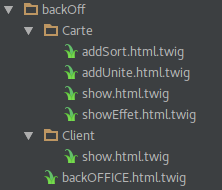
\includegraphics[scale=0.04]{Assets/backOff.png}~\\[1.5cm]

    \textsc{\LARGE IUT informatique de Belfort-Montbéliard}\\[2cm]

    \textsc{\Large Manuel utilisateur}\\[1.5cm]

    % Title
    \HRule \\[0.4cm]
    { \huge \bfseries Data wars\\[0.4cm] }

    \HRule \\[2cm]
    
\includegraphics[scale=0.4]{../mainPageimg.png}
    \\[2cm]

    % Author and supervisor
    \begin{minipage}{0.4\textwidth}
      \begin{flushleft} \large
        Guillaume \textsc{LAROYENNE}, \\ Nathan \textsc{PRETOT}, \\ Jeremy \textsc{RENAUD}, \\ Tom \textsc{SALVI}, \\ Pierre \textsc{VALENZA}
      \end{flushleft}
    \end{minipage}
    \begin{minipage}{0.4\textwidth}
      \begin{flushright} \large
        \emph{Tutrice :} Mme. \textsc{Deschinkel} \\
      \end{flushright}
    \end{minipage}

    \vfill

    % Bottom of the page
    {\large 1\ier{} Octobre 2016 — 27 Mars 2016}

  \end{center}
  \end{sffamily}
\end{titlepage}
\end{document}
